\documentclass{article}
\usepackage{tikz,times}
\usepackage[paperwidth=25cm,paperheight=22cm,left=1cm,top=1cm]{geometry}

\usetikzlibrary{mindmap,backgrounds}

\pagestyle{empty}

\begin{document}
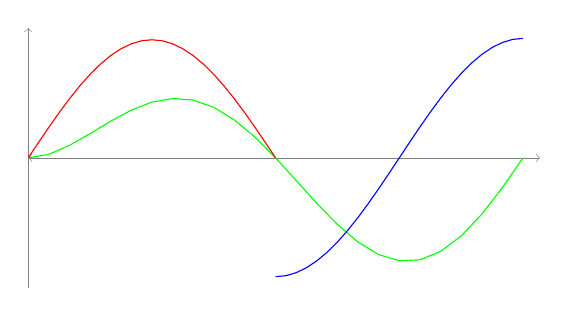
\begin{tikzpicture}[yscale=1.5]
\draw [help lines, <->]  (0,0) -- (6.5,0);
\draw [help lines, ->] (0,-1.1) -- (0,1.1);
\draw [green,domain=0:2*pi] plot (\x, {(sin(\x r)* ln(\x+1))/2});
\draw [red,domain=0:pi] plot (\x, {sin(\x r)});
\draw [blue, domain=pi:2*pi] plot (\x, {cos(\x r)*exp(\x/exp(2*pi))});
\end{tikzpicture}

\begin{tikzpicture}
\draw[<->] (6,0) node[below]{$q$} -- (0,0) --(0,6) node[left]{$V(q)$};
\draw[very thick] (0,0) to [out=90,in=0] (5,4.5);
\draw [thick] (0,5) to [out=-80, in=160] (3,.8) to[out=-20, in=175] (6,0);
\end{tikzpicture}

\end{document}
